\documentclass{standalone}
\usepackage{tikz}
\usetikzlibrary{patterns, positioning}

\begin{document}
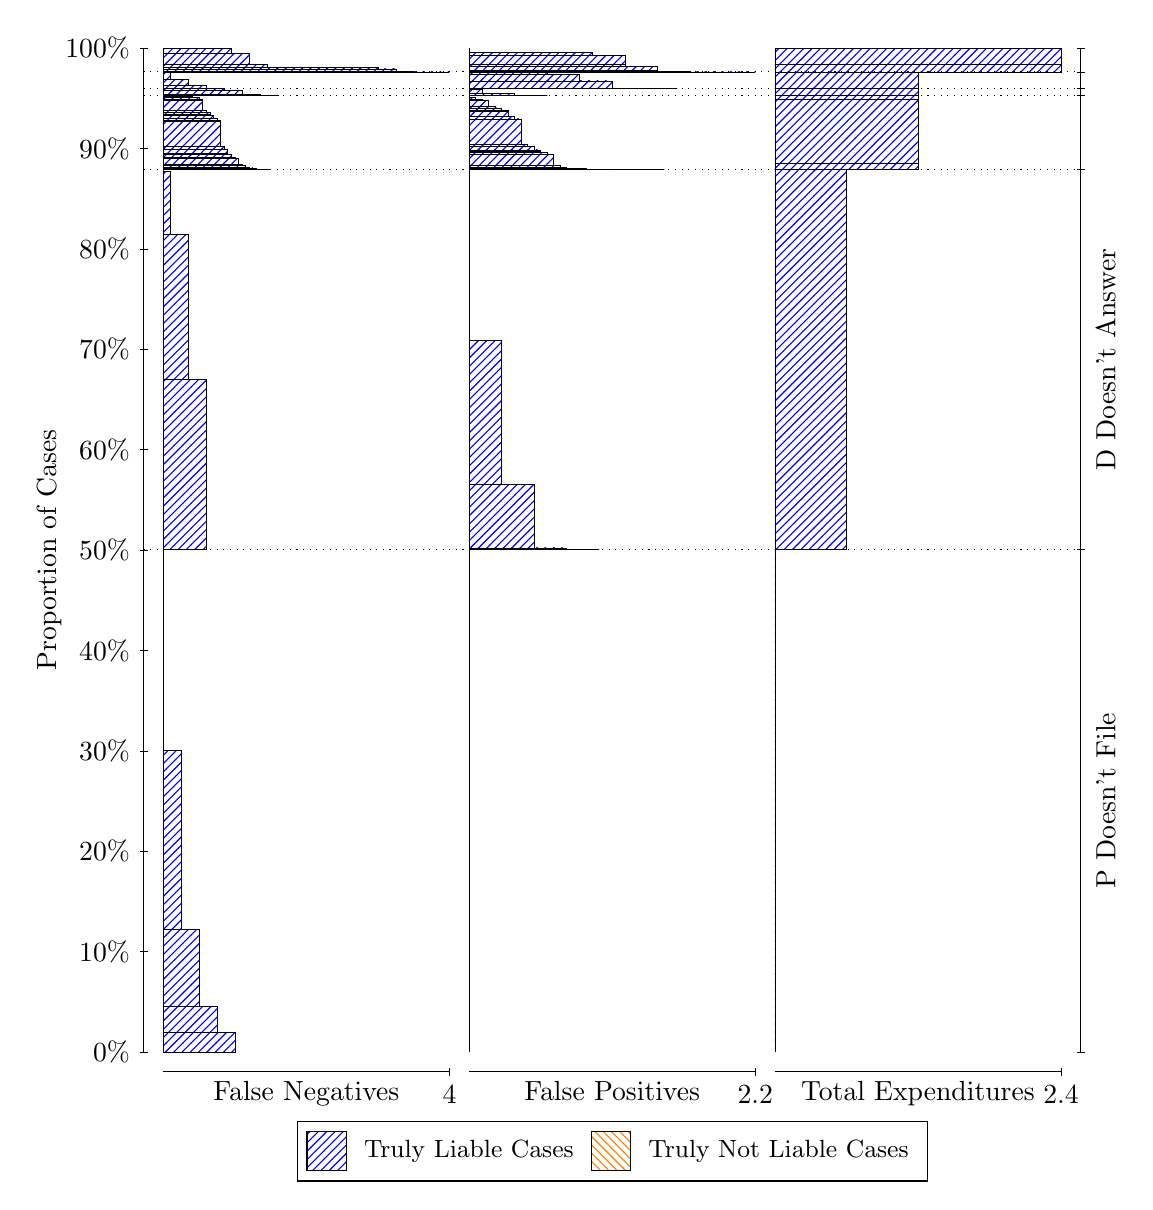
\begin{tikzpicture}
\draw[black, very thin] (1.5,1.75) -- (1.5,14.5);
\node[rotate=90, anchor=center] at (0.3, 8.125) {Proportion of Cases};
\draw[black, very thin] (1.45,1.75) -- (1.55,1.75);
\node[anchor=east] at (1.45, 1.75) {0\%};
\draw[black, very thin] (1.45,3.025) -- (1.55,3.025);
\node[anchor=east] at (1.45, 3.025) {10\%};
\draw[black, very thin] (1.45,4.3) -- (1.55,4.3);
\node[anchor=east] at (1.45, 4.3) {20\%};
\draw[black, very thin] (1.45,5.575) -- (1.55,5.575);
\node[anchor=east] at (1.45, 5.575) {30\%};
\draw[black, very thin] (1.45,6.85) -- (1.55,6.85);
\node[anchor=east] at (1.45, 6.85) {40\%};
\draw[black, very thin] (1.45,8.125) -- (1.55,8.125);
\node[anchor=east] at (1.45, 8.125) {50\%};
\draw[black, very thin] (1.45,9.4) -- (1.55,9.4);
\node[anchor=east] at (1.45, 9.4) {60\%};
\draw[black, very thin] (1.45,10.675) -- (1.55,10.675);
\node[anchor=east] at (1.45, 10.675) {70\%};
\draw[black, very thin] (1.45,11.95) -- (1.55,11.95);
\node[anchor=east] at (1.45, 11.95) {80\%};
\draw[black, very thin] (1.45,13.225) -- (1.55,13.225);
\node[anchor=east] at (1.45, 13.225) {90\%};
\draw[black, very thin] (1.45,14.5) -- (1.55,14.5);
\node[anchor=east] at (1.45, 14.5) {100\%};

\draw[black, very thin] (13.4,1.75) -- (13.4,14.5);
\draw[black, very thin] (13.35,1.75) -- (13.45,1.75);
\node[anchor=west] at (13.35, 1.75) {};
\draw[black, very thin] (13.35,8.1283) -- (13.45,8.1283);
\node[anchor=west] at (13.35, 8.1283) {};
\draw[black, very thin] (13.35,12.957) -- (13.45,12.957);
\node[anchor=west] at (13.35, 12.957) {};
\draw[black, very thin] (13.35,13.898) -- (13.45,13.898);
\node[anchor=west] at (13.35, 13.898) {};
\draw[black, very thin] (13.35,13.988) -- (13.45,13.988);
\node[anchor=west] at (13.35, 13.988) {};
\draw[black, very thin] (13.35,14.198) -- (13.45,14.198);
\node[anchor=west] at (13.35, 14.198) {};
\draw[black, very thin] (13.35,14.5) -- (13.45,14.5);
\node[anchor=west] at (13.35, 14.5) {};

\draw[black, very thin, pattern color=blue, pattern=north east lines] (1.75,1.75) rectangle (2.6583,1.9958);
\draw[black, very thin, pattern color=blue, pattern=north east lines] (1.75,1.9958) rectangle (2.4312,2.3295);
\draw[black, very thin, pattern color=blue, pattern=north east lines] (1.75,2.3295) rectangle (2.2042,3.3116);
\draw[black, very thin, pattern color=blue, pattern=north east lines] (1.75,3.3116) rectangle (1.9771,5.5811);
\draw[black, very thin, pattern color=orange, pattern=north west lines] (1.75,5.5811) rectangle (1.75,5.5811);
\draw[black, very thin, pattern color=blue, pattern=north east lines] (1.75,5.5811) rectangle (1.75,8.1283);
\draw[black, very thin, pattern color=blue, pattern=north east lines] (1.75,8.1283) rectangle (2.295,10.296);
\draw[black, very thin, pattern color=blue, pattern=north east lines] (1.75,10.296) rectangle (2.0679,12.13);
\draw[black, very thin, pattern color=blue, pattern=north east lines] (1.75,12.13) rectangle (1.8408,12.933);
\draw[black, very thin, pattern color=orange, pattern=north west lines] (1.75,12.933) rectangle (1.75,12.933);
\draw[black, very thin, pattern color=blue, pattern=north east lines] (1.75,12.933) rectangle (1.75,12.957);
\draw[black, very thin, pattern color=blue, pattern=north east lines] (1.75,12.957) rectangle (3.1125,12.959);
\draw[black, very thin, pattern color=blue, pattern=north east lines] (1.75,12.959) rectangle (3.0217,12.961);
\draw[black, very thin, pattern color=blue, pattern=north east lines] (1.75,12.961) rectangle (2.9308,12.967);
\draw[black, very thin, pattern color=blue, pattern=north east lines] (1.75,12.967) rectangle (2.8854,12.977);
\draw[black, very thin, pattern color=blue, pattern=north east lines] (1.75,12.977) rectangle (2.84,12.981);
\draw[black, very thin, pattern color=blue, pattern=north east lines] (1.75,12.981) rectangle (2.7946,13.008);
\draw[black, very thin, pattern color=blue, pattern=north east lines] (1.75,13.008) rectangle (2.7492,13.018);
\draw[black, very thin, pattern color=blue, pattern=north east lines] (1.75,13.018) rectangle (2.7037,13.094);
\draw[black, very thin, pattern color=blue, pattern=north east lines] (1.75,13.094) rectangle (2.6583,13.116);
\draw[black, very thin, pattern color=blue, pattern=north east lines] (1.75,13.116) rectangle (2.6129,13.15);
\draw[black, very thin, pattern color=blue, pattern=north east lines] (1.75,13.15) rectangle (2.5675,13.161);
\draw[black, very thin, pattern color=blue, pattern=north east lines] (1.75,13.161) rectangle (2.5675,13.219);
\draw[black, very thin, pattern color=blue, pattern=north east lines] (1.75,13.219) rectangle (2.5221,13.254);
\draw[black, very thin, pattern color=blue, pattern=north east lines] (1.75,13.254) rectangle (2.4767,13.575);
\draw[black, very thin, pattern color=blue, pattern=north east lines] (1.75,13.575) rectangle (2.4767,13.581);
\draw[black, very thin, pattern color=blue, pattern=north east lines] (1.75,13.581) rectangle (2.4312,13.61);
\draw[black, very thin, pattern color=blue, pattern=north east lines] (1.75,13.61) rectangle (2.3858,13.649);
\draw[black, very thin, pattern color=blue, pattern=north east lines] (1.75,13.649) rectangle (2.3404,13.662);
\draw[black, very thin, pattern color=blue, pattern=north east lines] (1.75,13.662) rectangle (2.3404,13.679);
\draw[black, very thin, pattern color=blue, pattern=north east lines] (1.75,13.679) rectangle (2.295,13.709);
\draw[black, very thin, pattern color=blue, pattern=north east lines] (1.75,13.709) rectangle (2.2496,13.839);
\draw[black, very thin, pattern color=blue, pattern=north east lines] (1.75,13.839) rectangle (2.2496,13.846);
\draw[black, very thin, pattern color=blue, pattern=north east lines] (1.75,13.846) rectangle (2.2042,13.872);
\draw[black, very thin, pattern color=blue, pattern=north east lines] (1.75,13.872) rectangle (2.1588,13.872);
\draw[black, very thin, pattern color=blue, pattern=north east lines] (1.75,13.872) rectangle (2.1588,13.88);
\draw[black, very thin, pattern color=blue, pattern=north east lines] (1.75,13.88) rectangle (2.1133,13.887);
\draw[black, very thin, pattern color=blue, pattern=north east lines] (1.75,13.887) rectangle (2.1133,13.887);
\draw[black, very thin, pattern color=blue, pattern=north east lines] (1.75,13.887) rectangle (2.0679,13.888);
\draw[black, very thin, pattern color=blue, pattern=north east lines] (1.75,13.888) rectangle (2.0225,13.89);
\draw[black, very thin, pattern color=blue, pattern=north east lines] (1.75,13.89) rectangle (2.0225,13.893);
\draw[black, very thin, pattern color=blue, pattern=north east lines] (1.75,13.893) rectangle (1.9771,13.894);
\draw[black, very thin, pattern color=blue, pattern=north east lines] (1.75,13.894) rectangle (1.9317,13.894);
\draw[black, very thin, pattern color=blue, pattern=north east lines] (1.75,13.894) rectangle (1.9317,13.898);
\draw[black, very thin, pattern color=blue, pattern=north east lines] (1.75,13.898) rectangle (1.8863,13.898);
\draw[black, very thin, pattern color=blue, pattern=north east lines] (1.75,13.898) rectangle (1.8408,13.898);
\draw[black, very thin, pattern color=blue, pattern=north east lines] (1.75,13.898) rectangle (1.7954,13.898);
\draw[black, very thin, pattern color=orange, pattern=north west lines] (1.75,13.898) rectangle (1.75,13.898);
\draw[black, very thin, pattern color=blue, pattern=north east lines] (1.75,13.898) rectangle (1.75,13.898);
\draw[black, very thin, pattern color=blue, pattern=north east lines] (1.75,13.898) rectangle (3.2033,13.901);
\draw[black, very thin, pattern color=blue, pattern=north east lines] (1.75,13.901) rectangle (2.9762,13.913);
\draw[black, very thin, pattern color=blue, pattern=north east lines] (1.75,13.913) rectangle (2.7492,13.962);
\draw[black, very thin, pattern color=blue, pattern=north east lines] (1.75,13.962) rectangle (2.5221,13.988);
\draw[black, very thin, pattern color=blue, pattern=north east lines] (1.75,13.988) rectangle (2.295,13.988);
\draw[black, very thin, pattern color=orange, pattern=north west lines] (1.75,13.988) rectangle (1.75,13.988);
\draw[black, very thin, pattern color=blue, pattern=north east lines] (1.75,13.988) rectangle (2.295,14.022);
\draw[black, very thin, pattern color=blue, pattern=north east lines] (1.75,14.022) rectangle (2.0679,14.102);
\draw[black, very thin, pattern color=blue, pattern=north east lines] (1.75,14.102) rectangle (1.8408,14.195);
\draw[black, very thin, pattern color=orange, pattern=north west lines] (1.75,14.195) rectangle (1.75,14.195);
\draw[black, very thin, pattern color=blue, pattern=north east lines] (1.75,14.195) rectangle (1.75,14.198);
\draw[black, very thin, pattern color=blue, pattern=north east lines] (1.75,14.198) rectangle (5.3833,14.198);
\draw[black, very thin, pattern color=blue, pattern=north east lines] (1.75,14.198) rectangle (5.1563,14.198);
\draw[black, very thin, pattern color=blue, pattern=north east lines] (1.75,14.198) rectangle (4.9292,14.202);
\draw[black, very thin, pattern color=blue, pattern=north east lines] (1.75,14.202) rectangle (4.7021,14.234);
\draw[black, very thin, pattern color=blue, pattern=north east lines] (1.75,14.234) rectangle (4.475,14.252);
\draw[black, very thin, pattern color=blue, pattern=north east lines] (1.75,14.252) rectangle (4.2479,14.252);
\draw[black, very thin, pattern color=blue, pattern=north east lines] (1.75,14.252) rectangle (4.0208,14.252);
\draw[black, very thin, pattern color=blue, pattern=north east lines] (1.75,14.252) rectangle (3.5213,14.252);
\draw[black, very thin, pattern color=blue, pattern=north east lines] (1.75,14.252) rectangle (3.2942,14.253);
\draw[black, very thin, pattern color=blue, pattern=north east lines] (1.75,14.253) rectangle (3.0671,14.295);
\draw[black, very thin, pattern color=blue, pattern=north east lines] (1.75,14.295) rectangle (2.84,14.435);
\draw[black, very thin, pattern color=blue, pattern=north east lines] (1.75,14.435) rectangle (2.6129,14.495);
\draw[black, very thin, pattern color=blue, pattern=north east lines] (1.75,14.495) rectangle (2.3858,14.5);
\draw[black, very thin, pattern color=blue, pattern=north east lines] (1.75,14.5) rectangle (2.1588,14.5);
\draw[black, very thin, pattern color=blue, pattern=north east lines] (1.75,14.5) rectangle (1.9317,14.5);
\draw[black, very thin, pattern color=orange, pattern=north west lines] (1.75,14.5) rectangle (1.75,14.5);
\draw[black, very thin, pattern color=orange, pattern=north west lines] (5.6333,1.75) rectangle (5.6333,1.75);
\draw[black, very thin, pattern color=blue, pattern=north east lines] (5.6333,1.75) rectangle (5.6333,8.1283);
\draw[black, very thin, pattern color=orange, pattern=north west lines] (5.6333,8.1283) rectangle (7.2848,8.1283);
\draw[black, very thin, pattern color=blue, pattern=north east lines] (5.6333,8.1283) rectangle (7.2848,8.1283);
\draw[black, very thin, pattern color=blue, pattern=north east lines] (5.6333,8.1283) rectangle (6.872,8.1529);
\draw[black, very thin, pattern color=blue, pattern=north east lines] (5.6333,8.1529) rectangle (6.4591,8.9553);
\draw[black, very thin, pattern color=blue, pattern=north east lines] (5.6333,8.9553) rectangle (6.0462,10.79);
\draw[black, very thin, pattern color=blue, pattern=north east lines] (5.6333,10.79) rectangle (5.6333,12.957);
\draw[black, very thin, pattern color=orange, pattern=north west lines] (5.6333,12.957) rectangle (8.1106,12.957);
\draw[black, very thin, pattern color=blue, pattern=north east lines] (5.6333,12.957) rectangle (8.1106,12.957);
\draw[black, very thin, pattern color=orange, pattern=north west lines] (5.6333,12.957) rectangle (7.9455,12.957);
\draw[black, very thin, pattern color=blue, pattern=north east lines] (5.6333,12.957) rectangle (7.9455,12.957);
\draw[black, very thin, pattern color=orange, pattern=north west lines] (5.6333,12.957) rectangle (7.7803,12.957);
\draw[black, very thin, pattern color=blue, pattern=north east lines] (5.6333,12.957) rectangle (7.7803,12.957);
\draw[black, very thin, pattern color=blue, pattern=north east lines] (5.6333,12.957) rectangle (7.6977,12.957);
\draw[black, very thin, pattern color=orange, pattern=north west lines] (5.6333,12.957) rectangle (7.6152,12.957);
\draw[black, very thin, pattern color=blue, pattern=north east lines] (5.6333,12.957) rectangle (7.6152,12.957);
\draw[black, very thin, pattern color=blue, pattern=north east lines] (5.6333,12.957) rectangle (7.5326,12.958);
\draw[black, very thin, pattern color=orange, pattern=north west lines] (5.6333,12.958) rectangle (7.45,12.958);
\draw[black, very thin, pattern color=blue, pattern=north east lines] (5.6333,12.958) rectangle (7.45,12.958);
\draw[black, very thin, pattern color=blue, pattern=north east lines] (5.6333,12.958) rectangle (7.3674,12.958);
\draw[black, very thin, pattern color=orange, pattern=north west lines] (5.6333,12.958) rectangle (7.2848,12.958);
\draw[black, very thin, pattern color=blue, pattern=north east lines] (5.6333,12.958) rectangle (7.2848,12.961);
\draw[black, very thin, pattern color=blue, pattern=north east lines] (5.6333,12.961) rectangle (7.2023,12.962);
\draw[black, very thin, pattern color=orange, pattern=north west lines] (5.6333,12.962) rectangle (7.1197,12.962);
\draw[black, very thin, pattern color=blue, pattern=north east lines] (5.6333,12.962) rectangle (7.1197,12.967);
\draw[black, very thin, pattern color=blue, pattern=north east lines] (5.6333,12.967) rectangle (7.0371,12.968);
\draw[black, very thin, pattern color=orange, pattern=north west lines] (5.6333,12.968) rectangle (6.9545,12.968);
\draw[black, very thin, pattern color=blue, pattern=north east lines] (5.6333,12.968) rectangle (6.9545,12.968);
\draw[black, very thin, pattern color=blue, pattern=north east lines] (5.6333,12.968) rectangle (6.9545,12.975);
\draw[black, very thin, pattern color=blue, pattern=north east lines] (5.6333,12.975) rectangle (6.872,12.983);
\draw[black, very thin, pattern color=orange, pattern=north west lines] (5.6333,12.983) rectangle (6.7894,12.983);
\draw[black, very thin, pattern color=blue, pattern=north east lines] (5.6333,12.983) rectangle (6.7894,13.009);
\draw[black, very thin, pattern color=blue, pattern=north east lines] (5.6333,13.009) rectangle (6.7068,13.146);
\draw[black, very thin, pattern color=blue, pattern=north east lines] (5.6333,13.146) rectangle (6.6242,13.177);
\draw[black, very thin, pattern color=blue, pattern=north east lines] (5.6333,13.177) rectangle (6.5417,13.193);
\draw[black, very thin, pattern color=blue, pattern=north east lines] (5.6333,13.193) rectangle (6.5417,13.206);
\draw[black, very thin, pattern color=blue, pattern=north east lines] (5.6333,13.206) rectangle (6.4591,13.246);
\draw[black, very thin, pattern color=blue, pattern=north east lines] (5.6333,13.246) rectangle (6.3765,13.274);
\draw[black, very thin, pattern color=blue, pattern=north east lines] (5.6333,13.274) rectangle (6.2939,13.601);
\draw[black, very thin, pattern color=blue, pattern=north east lines] (5.6333,13.601) rectangle (6.2114,13.636);
\draw[black, very thin, pattern color=blue, pattern=north east lines] (5.6333,13.636) rectangle (6.1288,13.695);
\draw[black, very thin, pattern color=blue, pattern=north east lines] (5.6333,13.695) rectangle (6.1288,13.706);
\draw[black, very thin, pattern color=blue, pattern=north east lines] (5.6333,13.706) rectangle (6.0462,13.74);
\draw[black, very thin, pattern color=blue, pattern=north east lines] (5.6333,13.74) rectangle (5.9636,13.762);
\draw[black, very thin, pattern color=blue, pattern=north east lines] (5.6333,13.762) rectangle (5.8811,13.837);
\draw[black, very thin, pattern color=blue, pattern=north east lines] (5.6333,13.837) rectangle (5.7985,13.847);
\draw[black, very thin, pattern color=blue, pattern=north east lines] (5.6333,13.847) rectangle (5.7159,13.874);
\draw[black, very thin, pattern color=blue, pattern=north east lines] (5.6333,13.874) rectangle (5.6333,13.898);
\draw[black, very thin, pattern color=orange, pattern=north west lines] (5.6333,13.898) rectangle (6.6242,13.898);
\draw[black, very thin, pattern color=blue, pattern=north east lines] (5.6333,13.898) rectangle (6.6242,13.898);
\draw[black, very thin, pattern color=blue, pattern=north east lines] (5.6333,13.898) rectangle (6.2114,13.924);
\draw[black, very thin, pattern color=blue, pattern=north east lines] (5.6333,13.924) rectangle (5.7985,13.973);
\draw[black, very thin, pattern color=blue, pattern=north east lines] (5.6333,13.973) rectangle (5.6333,13.988);
\draw[black, very thin, pattern color=orange, pattern=north west lines] (5.6333,13.988) rectangle (8.2758,13.988);
\draw[black, very thin, pattern color=blue, pattern=north east lines] (5.6333,13.988) rectangle (8.2758,13.988);
\draw[black, very thin, pattern color=blue, pattern=north east lines] (5.6333,13.988) rectangle (7.8629,13.991);
\draw[black, very thin, pattern color=blue, pattern=north east lines] (5.6333,13.991) rectangle (7.45,14.084);
\draw[black, very thin, pattern color=blue, pattern=north east lines] (5.6333,14.084) rectangle (7.0371,14.164);
\draw[black, very thin, pattern color=blue, pattern=north east lines] (5.6333,14.164) rectangle (6.6242,14.198);
\draw[black, very thin, pattern color=orange, pattern=north west lines] (5.6333,14.198) rectangle (9.2667,14.198);
\draw[black, very thin, pattern color=blue, pattern=north east lines] (5.6333,14.198) rectangle (9.2667,14.198);
\draw[black, very thin, pattern color=blue, pattern=north east lines] (5.6333,14.198) rectangle (8.8538,14.198);
\draw[black, very thin, pattern color=orange, pattern=north west lines] (5.6333,14.198) rectangle (8.8538,14.198);
\draw[black, very thin, pattern color=blue, pattern=north east lines] (5.6333,14.198) rectangle (8.8538,14.198);
\draw[black, very thin, pattern color=blue, pattern=north east lines] (5.6333,14.198) rectangle (8.4409,14.201);
\draw[black, very thin, pattern color=orange, pattern=north west lines] (5.6333,14.201) rectangle (8.4409,14.201);
\draw[black, very thin, pattern color=blue, pattern=north east lines] (5.6333,14.201) rectangle (8.4409,14.203);
\draw[black, very thin, pattern color=blue, pattern=north east lines] (5.6333,14.203) rectangle (8.028,14.217);
\draw[black, very thin, pattern color=orange, pattern=north west lines] (5.6333,14.217) rectangle (8.028,14.217);
\draw[black, very thin, pattern color=blue, pattern=north east lines] (5.6333,14.217) rectangle (8.028,14.263);
\draw[black, very thin, pattern color=blue, pattern=north east lines] (5.6333,14.263) rectangle (7.6152,14.291);
\draw[black, very thin, pattern color=blue, pattern=north east lines] (5.6333,14.291) rectangle (7.6152,14.404);
\draw[black, very thin, pattern color=blue, pattern=north east lines] (5.6333,14.404) rectangle (7.2023,14.445);
\draw[black, very thin, pattern color=blue, pattern=north east lines] (5.6333,14.445) rectangle (6.7894,14.447);
\draw[black, very thin, pattern color=blue, pattern=north east lines] (5.6333,14.447) rectangle (6.3765,14.447);
\draw[black, very thin, pattern color=orange, pattern=north west lines] (5.6333,14.447) rectangle (5.6333,14.447);
\draw[black, very thin, pattern color=blue, pattern=north east lines] (5.6333,14.447) rectangle (5.6333,14.5);
\draw[black, very thin, pattern color=orange, pattern=north west lines] (9.5167,1.75) rectangle (9.5167,1.75);
\draw[black, very thin, pattern color=blue, pattern=north east lines] (9.5167,1.75) rectangle (9.5167,8.1283);
\draw[black, very thin, pattern color=orange, pattern=north west lines] (9.5167,8.1283) rectangle (10.425,8.1283);
\draw[black, very thin, pattern color=blue, pattern=north east lines] (9.5167,8.1283) rectangle (10.425,12.957);
\draw[black, very thin, pattern color=orange, pattern=north west lines] (9.5167,12.957) rectangle (11.333,12.957);
\draw[black, very thin, pattern color=blue, pattern=north east lines] (9.5167,12.957) rectangle (11.333,13.033);
\draw[black, very thin, pattern color=orange, pattern=north west lines] (9.5167,13.033) rectangle (11.333,13.033);
\draw[black, very thin, pattern color=blue, pattern=north east lines] (9.5167,13.033) rectangle (11.333,13.85);
\draw[black, very thin, pattern color=orange, pattern=north west lines] (9.5167,13.85) rectangle (11.333,13.85);
\draw[black, very thin, pattern color=blue, pattern=north east lines] (9.5167,13.85) rectangle (11.333,13.898);
\draw[black, very thin, pattern color=orange, pattern=north west lines] (9.5167,13.898) rectangle (11.333,13.898);
\draw[black, very thin, pattern color=blue, pattern=north east lines] (9.5167,13.898) rectangle (11.333,13.988);
\draw[black, very thin, pattern color=orange, pattern=north west lines] (9.5167,13.988) rectangle (11.333,13.988);
\draw[black, very thin, pattern color=blue, pattern=north east lines] (9.5167,13.988) rectangle (11.333,14.198);
\draw[black, very thin, pattern color=orange, pattern=north west lines] (9.5167,14.198) rectangle (13.15,14.198);
\draw[black, very thin, pattern color=blue, pattern=north east lines] (9.5167,14.198) rectangle (13.15,14.296);
\draw[black, very thin, pattern color=orange, pattern=north west lines] (9.5167,14.296) rectangle (13.15,14.296);
\draw[black, very thin, pattern color=blue, pattern=north east lines] (9.5167,14.296) rectangle (13.15,14.5);
\draw[black, dotted] (1.5,8.1283) -- (13.4,8.1283);
\draw[black, dotted] (1.5,12.957) -- (13.4,12.957);
\draw[black, dotted] (1.5,13.898) -- (13.4,13.898);
\draw[black, dotted] (1.5,13.988) -- (13.4,13.988);
\draw[black, dotted] (1.5,14.198) -- (13.4,14.198);
\draw[black, very thin] (1.75,1.5) -- (5.3833,1.5);
\node[anchor=north] at (3.5667, 1.5) {False Negatives};
\draw[black, very thin] (5.3833,1.45) -- (5.3833,1.55);
\node[anchor=north] at (5.3833, 1.45) {4};

\draw[black, very thin] (5.6333,1.5) -- (9.2667,1.5);
\node[anchor=north] at (7.45, 1.5) {False Positives};
\draw[black, very thin] (9.2667,1.45) -- (9.2667,1.55);
\node[anchor=north] at (9.2667, 1.45) {2.2};

\draw[black, very thin] (9.5167,1.5) -- (13.15,1.5);
\node[anchor=north] at (11.333, 1.5) {Total Expenditures};
\draw[black, very thin] (13.15,1.45) -- (13.15,1.55);
\node[anchor=north] at (13.15, 1.45) {2.4};

\node[black, centered, rotate=90] at (13.72, 4.9391) {P Doesn't File};
\node[black, centered, rotate=90] at (13.72, 10.543) {D Doesn't Answer};





\draw (7.449999999999999,1.5) node[draw=none] (baseCoordinate) {};
\begin{scope}[align=center]
        \matrix[scale=0.5, draw=black, below=0.5cm of baseCoordinate, nodes={draw}, column sep=0.1cm]{
            \node[rectangle, draw, minimum width=0.5cm, minimum height=0.5cm, pattern=north east lines, pattern color=blue] {}; &
            \node[draw=none, font=\small] (B) {Truly Liable Cases}; &
            \node[rectangle, draw, minimum width=0.5cm, minimum height=0.5cm, pattern=north west lines, pattern color=orange] {}; &
            \node[draw=none, font=\small] (B) {Truly Not Liable Cases}; \\
            };
\end{scope}

\end{tikzpicture}
\end{document}